%
% File emnlp2020.tex
%
%% Based on the style files for ACL 2020, which were
%% Based on the style files for ACL 2018, NAACL 2018/19, which were
%% Based on the style files for ACL-2015, with some improvements
%%  taken from the NAACL-2016 style
%% Based on the style files for ACL-2014, which were, in turn,
%% based on ACL-2013, ACL-2012, ACL-2011, ACL-2010, ACL-IJCNLP-2009,
%% EACL-2009, IJCNLP-2008...
%% Based on the style files for EACL 2006 by 
%%e.agirre@ehu.es or Sergi.Balari@uab.es
%% and that of ACL 08 by Joakim Nivre and Noah Smith

\documentclass[11pt,a4paper]{article}
\usepackage[hyperref]{emnlp2020}
\usepackage{times}
\usepackage{latexsym}
\usepackage{graphicx}
\usepackage{amsmath}
\usepackage{amssymb}
\usepackage{multirow}
\usepackage{pgfplots}
\usepackage{booktabs}
\usepackage{subfigure}
\usepackage{xcolor}
\usepackage{comment}
\usepackage{bm}
\usepackage{url}
\pgfplotsset{width=0.9\columnwidth,compat=1.9}

\renewcommand{\UrlFont}{\ttfamily\small}

% This is not strictly necessary, and may be commented out,
% but it will improve the layout of the manuscript,
% and will typically save some space.
\usepackage{microtype}

\definecolor{mygreen}{rgb}{0.372822,0.630254,0.217202}
\definecolor{myblue}{rgb}{0.208317,0.357233,0.717412}
\definecolor{myorange}{rgb}{1,0.5,0}
\aclfinalcopy% Uncomment this line for the final submission
%\def\aclpaperid{***} %  Enter the acl Paper ID here

%\setlength\titlebox{5cm}
% You can expand the titlebox if you need extra space
% to show all the authors. Please do not make the titlebox
% smaller than 5cm (the original size); we will check this
% in the camera-ready version and ask you to change it back.

\newcommand\BibTeX{B\textsc{ib}\TeX}

\title{Language Generation with Multi-Hop Reasoning on Commonsense Knowledge Graph}

\author{Haozhe Ji$^1$, Pei Ke$^1$, Shaohan Huang$^2$, Furu Wei$^2$, Xiaoyan Zhu$^1$, Minlie Huang$^1$\thanks{\quad Corresponding author}  \\
$^1$Department of Computer Science and Technology,
Institute for Artificial Intelligence, \\
State Key Lab of Intelligent Technology and Systems, \\ 
Beijing National Research Center for Information Science and Technology, \\ 
Tsinghua University, Beijing 100084, China \\
$^2$Microsoft Research \\
  {\tt\small \{jhz20,kp17\}@mails.tsinghua.edu.cn, \{shaohanh, fuwei\}@microsoft.com, } \\
  {\tt\small \{zxy-dcs,aihuang\}@tsinghua.edu.cn } \\}

\date{}

\begin{document}
\maketitle
\begin{abstract}
Despite the success of generative pre-trained language models on a series of text generation tasks, they still suffer in cases where reasoning over underlying commonsense knowledge is required during generation.
Existing approaches that integrate commonsense knowledge into generative pre-trained language models simply transfer relational knowledge by post-training on individual knowledge triples while ignoring rich connections within the knowledge graph. We argue that exploiting both the structural and semantic information of the knowledge graph facilitates commonsense-aware text generation. In this paper, we propose \textit{Generation with Multi-Hop Reasoning Flow} (GRF) that enables pre-trained models with dynamic multi-hop reasoning on multi-relational paths extracted from the external commonsense knowledge graph. We empirically show that our model outperforms existing baselines on three text generation tasks that require reasoning over commonsense knowledge. We also demonstrate the effectiveness of the dynamic multi-hop reasoning module with reasoning paths inferred by the model that provide rationale to the generation.\footnote{The source code is available at \url{https://github.com/cdjhz/multigen}.}
\end{abstract}

\section{Introduction}
%Equipping machine with commonsense reasoning ability has been acknowledged as a crucial indicator in artificial intelligence~\citep{Davis2015CommonsenseRA}. So far a considerable amount of work has been dedicated to evaluate this ability from various aspects. A majority of these tasks ask models to draw inferences~\citep{Levesque2011TheWS, Zellers2018SWAGAL} or make choices from multiple plausible candidates~\citep{Talmor2018CommonsenseQAAQ, Huang2019CosmosQM, Sap2019SocialIC} in a discriminative way. Our interest primarily lies in empowering the generation model with reasoning ability grounding on commonsense knowledge. 
%Commonsense reasoning requires utilizing basic knowledge that reflects human's natural understanding to the world to solve complex reasoning problems.
Despite the recent success of pre-trained language models such as GPT-2~\citep{Radford2019LanguageMA} on various language generation tasks, these models are still struggling on generation tasks that require reasoning over commonsense knowledge that is not \textit{explicitly} stated in the context. 
%% relational knowledge 一般指三元组形式的关系性知识
For example, Figure \ref{fig:example} illustrates an example in the story ending generation task, where external commonsense knowledge in the form of relational paths %forms multi-hop paths that 
can guide the generation of the key concepts ``substance'' and ``lava'' in the story ending by providing background knowledge such as $(\texttt{volcano}, \texttt{MadeOf}, \texttt{lava})$ besides the story context. Although pre-trained models have been demonstrated to 
%recall relational facts~\citep{Lama2019, bouraoui2019inducing} or 
possess commonsense 
reasoning ability~\citep{Trinh2018ASM} by \textit{implicitly} learning some relational patterns from large-scale corpora, they do not fully utilize the commonsense knowledge bases that provide more explicit knowledge grounding.


%Although these models have been demonstrated to recall relational facts~\citep{Lama2019, bouraoui2019inducing} or possess commonsense discrimination ability~\citep{Trinh2018ASM} benefiting from optimizing text-based self-supervised objectives, it is not clear whether they are making interpretable inferences or capturing dubious biases in the datasets~\citep{niven-kao-2019-probing}.%without explicitly grounding on well-defined commonsense knowledge. 

\begin{figure}
    \centering
    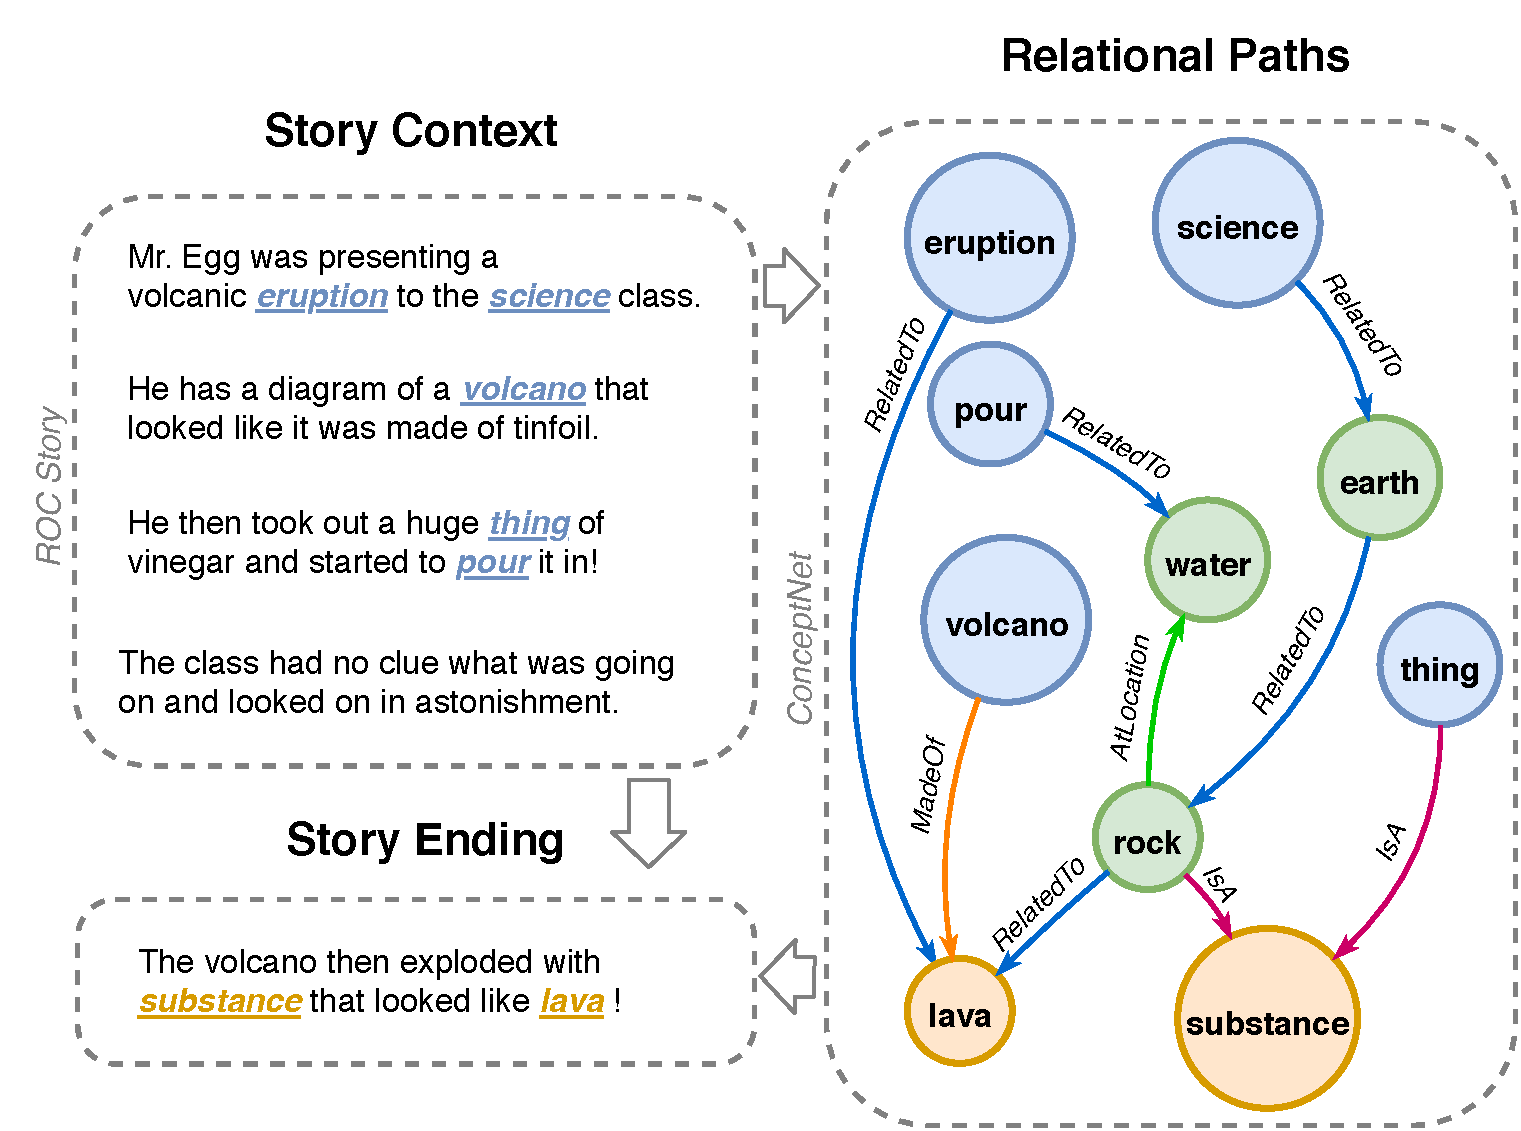
\includegraphics[width=1.0\columnwidth]{story_example3.pdf}
    \caption{An example of using structural relational knowledge as commonsense grounding in story ending generation. \textcolor{myblue}{Blue nodes} correspond to the concepts in the context, \textcolor{myorange}{orange nodes} correspond to those in the
    story ending and \textcolor{mygreen}{gree nodes} are intermediate concepts that connect the evidence chain.}
    \label{fig:example}
\end{figure}

To address this defect, incorporating external commonsense knowledge to enhance models' reasoning ability has been widely explored~\citep{lin-etal-2019-kagnet,Ye2019AlignMA,Lv2020GraphBasedRO}.
%%%shiyang这个参考文献格式错误？看起来不是姓
In language generation, previous work~\citep{Bhagavatula2019AbductiveCR, guan2020knowledge} transfers commonsense knowledge into pre-trained language models by utilizing triple information in commonsense knowledge bases such as ConceptNet~\citep{Speer2012RepresentingGR} and ATOMIC~\citep{Sap2019ATOMICAA}. %In this manner, the models learn relational knowledge \textit{implicitly} by capturing semantic relations in natural language text. 

However, this approach has two drawbacks. 
% give an example
First, recovering knowledge triples at the post-training stage~\citep{guan2020knowledge} hardly enables the model to utilize the encoded knowledge in fine-tuning generation tasks which requires reasoning over underlying commonsense knowledge.
%for grounded text generation.
%then fine-tuning on task data explicitly reason over evidences for grounded text generation which is less promising.
Second, it ignores the abundant structural relational relevance of the concepts in the knowledge graph~\citep{guan2020knowledge,Bhagavatula2019AbductiveCR} that may provide multiple plausible evidence for complex reasoning. 
%lays a heavy burden on the generation model to re-contextualize the encoded knowledge in the learned representations. 
%Due to the incompleteness nature of knowledge bases~\citep{Min2013DistantSF}, evidence directly linking pairs of entities in most realistic generation tasks is not always available and therefore leveraging multi-hop connections is a more desirable way~\citep{McCallum2017ChainsOR,Das2018GoFA,Stadelmaier2019ModelingPF}. 
%(However, the model may infer some likelihood from multi-hop linkings). 
Thus a richer and more explicit way of utilizing external commonsense knowledge is to exploit both \textit{structural} and \textit{semantic} information of the knowledge graph and reason over multi-hop relational paths where multiple connected triples provide chains of evidence for grounded text generation.
%%%% 此处 semantic information 指单个 triple 所体现的语义信息，structural information 则是指多跳结构带来的信息
%support the generation of some key mentions.% conditioned on contexts. 

In this paper, we propose \textit{Generation with Multi-Hop Reasoning Flow} (GRF), a generation model that performs multi-hop reasoning on the external knowledge graph for knowledge-enriched language generation.
%involves reasoning on external knowledge graph by performing  when generating each token. 
The model operates on the sub-graph extended from the concepts in the input text as commonsense knowledge grounding. It first encodes the multi-relational graph with compositional operation to obtain graph-aware representations for the concepts and the relations (\S{\ref{sec:static-graph}}). 
Then, the multi-hop reasoning module performs dynamic reasoning via aggregating triple evidence along multiple relational paths %(from \textit{source nodes}) 
%via scored edges %that consider relational information 
%from the concepts to all the concepts on the subgraph 
to generate the salient concept under the context (\S{\ref{sec:dmrf}}). 
%We explore several representational techniques of encoding the relational information of each triplet that forms a single piece of evidence in the path.
Finally, the generation distribution combines the probability of copying concepts from the knowledge graph and that of choosing a word from the standard vocabulary with a gate control (\S{\ref{sec:gate}}). The overall model architecture is shown in Figure \ref{fig:model}. 
%%%%hml上面这段写得不太好
We conduct experiments on three commonsense-aware text generation tasks
%tasks that requires commonsense reasoning 
including story ending generation~\citep{Mostafazadeh2016ACA}, abductive natural language generation~\citep{Bhagavatula2019AbductiveCR}, and explanation generation for sense making~\citep{Wang2019DoesIM}. 
Results show that our model outperforms strong baselines on these tasks, thereby demonstrating the benefit of multi-hop commonsense reasoning in language generation.

%Figure \ref{fig:example} illustrates how the GSF utilizes both semantic context and symbolic paths during generation. A series of paths extend from the \textit{source nodes} extracted from the context to build symbolic connections with the target mentions, i.e. ``substance'' and ``lava'' in the story ending. When generating ``lava'', likelihood propagates from \textit{source nodes} via chains of evidence such as (\texttt{volcano}, \texttt{MadeOf}, \texttt{lava}) to activate the node representing ``lava''.

%Similar to story ending generation where additional relational commonsense knowledge provides evidence that connects the story context to the ending, 
%%%%Similar to story ending generation, in abductive natural language generation and explanation generation we can also construct relational paths that connect from observation to hypothesis and statement to explanation respectively to support the evidence flow. 

Our contributions can be summarized as follows: 1) We propose GRF, a novel generation model that utilizes external structural commonsense knowledge to facilitate explicit commonsense reasoning in text generation. 2) We propose the dynamic multi-hop reasoning module that 
%integrates structural graph embeddings and textual representations and 
aggregates evidence along relational paths for grounded generation of some critical concepts.
3) We conduct extensive experiments including automatic and human evaluation on three commonsense-aware text generation tasks and show that our model outperforms various selective baselines. We also visualize reasoning paths inferred by the model to demonstrate the effectiveness of the multi-hop reasoning module. 
%3) We demonstrate the effectiveness of the dynamic multi-hop reasoning module and provide inferred reasoning paths to show how the model utilizes multi-hop evidence to support the generation of some key concepts.
%This approach however has the following drawbacks. (1) 
%Problem of post-training:
%(1) no explicit reasoning with the commonsense knowledge
%(2) catastrophic forgetting problem of post-training, heavily relies on model %capacity
%(3) implicit reasoning not explainable, dubious generation
%(4) Fine-grained control 

%Handle multi-hop problem

\begin{figure*}[t]
    \centering
    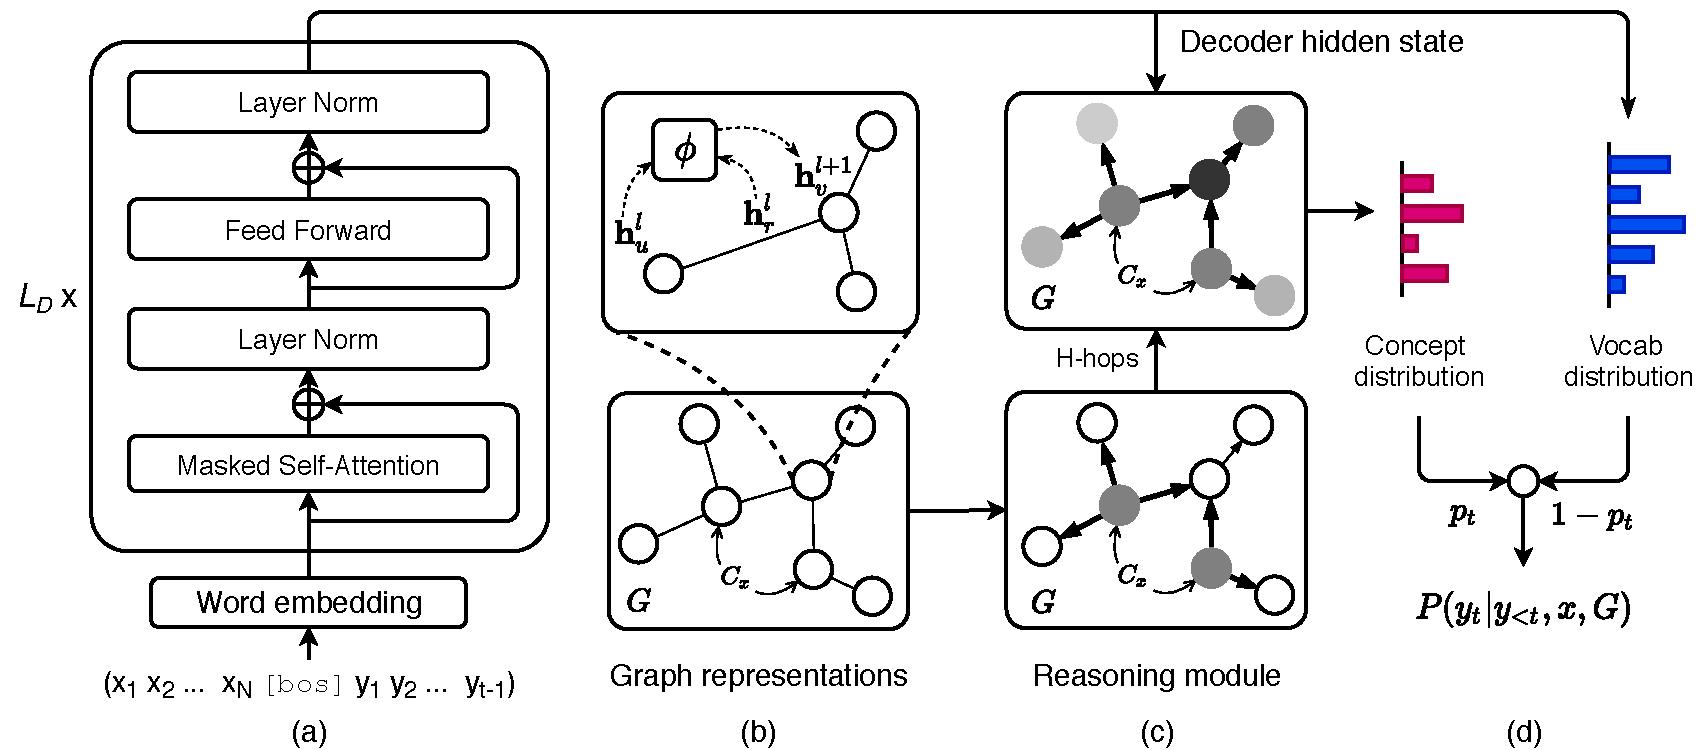
\includegraphics[width=1.7\columnwidth]{model_arch3.pdf}
    \caption{Model architecture. (a) Context modeling with pre-trained transformer (\S{\ref{sec:text}}). (b) The model encodes the multi-relational graph with non-parametric operation $\phi(\cdot)$ to combine relations and concepts (\S{\ref{sec:static-graph}}). %%%compositional operation 这个词不准确，组合，合成，是指短变长的过程
    (c) The multi-hop reasoning module aggregates evidence from source concepts $C_{\bm{x}}$ along structural paths to all nodes where shade indicates the node score (\S{\ref{sec:dmrf}}). (d) 
   The final generation distribution with gate control (\S{\ref{sec:gate}}).}
    \label{fig:model}
\end{figure*}
%%%图上dist. --> distribution 又不是没有空间

\section{Related Work}
\subsection{Commonsense-Aware Neural Text Generation}
Incorporating commonsense knowledge is essential for text generation to 
%enhance model's reasoning capability beyond 
augment the limited textual information. In dialogue generation, \citet{Zhou2018CommonsenseKA} enriched the context representations of the post with neighbouring concepts on ConceptNet using graph attention. In story ending generation, \citet{Guan2019StoryEG} proposed incremental encoding with multi-source attention to incorporate one-hop knowledge graph for concepts in the story context.
%enriches the context representaton of the story with a similar graph attention mechanism to the related concepts. 
In topic-to-essay generation, \citet{yang-etal-2019-enhancing-topic} augmented the generator with a concept memory that updated dynamically with gate mechanism.
Recently, some work also attempted to integrate external commonsense knowledge into generative pre-trained language models such as GPT-2~\citep{Radford2019LanguageMA}. \citet{guan2020knowledge} conducted post-training on sythetic data constructed from commonsense knowledge bases by translating triplets into natural language texts using templates. \citet{Bhagavatula2019AbductiveCR} transferred embeddings of COMeT~\citep{Bosselut2019COMETCT}, a GPT-2 model fine-tuned to 
generate the tail entity of a triple in commonsense knowledge graph, into another GPT-2 model for text generation. In comparison, our model utilizes both structural and semantic information of the commonsense knowledge graph during generation and does not suffers from the catastrophic forgetting problem~\citep{Kirkpatrick2016OvercomingCF} caused by implicit knowledge transferring.

\subsection{Multi-Hop Reasoning on Graph Structure}
Performing explicit multi-hop reasoning on graph structure has been demonstrated to be an effective approach for query answering over incomplete knowledge graphs~\citep{Das2018GoFA, Chen2018VariationalKG, Lin2018MultiHopKG}, multi-hop question answering~\citep{Bauer2018CommonsenseFG,Cao2018QuestionAB,Xiao2019DynamicallyFG} and dialogue generation~\citep{Tuan2019DyKgChatBD,Moon2019OpenDialKGEC, Liu2019KnowledgeAC}. Particularly, reasoning on knowledge graphs to answer relational query typically adopts REINFORCE to learn concrete policies to search for entities or relations. In multi-hop question answering tasks, the reasoning process is augmented with entity graph~\citep{Cao2018QuestionAB,Xiao2019DynamicallyFG} or concept paths~\citep{Bauer2018CommonsenseFG} to enhance semantic connections among document segments. 
%Combining multi-hop reasoning with the generation model is mostly explored in the dialogue generation task. 
In dialogue generation, \citet{Tuan2019DyKgChatBD} modeled multiple hops on relationship graphs with a Markov transition matrix. \citet{Liu2019KnowledgeAC} proposed a two-stage architecture that selected information from a knowledge graph for further generating the response. Compared with these generation models that operate on knowledge graphs within a specific domain, our focus is to utilize general commonsense knowledge to supply evidence for text generation.
%and emphasiz commonsense reasoning in text generation.

\section{Methodology}



\subsection{Problem Formulation}

In this paper, we focus on text generation tasks where reasoning over external commonsense knowledge is required. Without loss of generality, the input source is a text sequence $\bm{x}=(x_1,x_2,\cdots, x_N)$ which may consist of several sentences. The output target is another text sequence $\bm{y}=(y_1,y_2,\cdots,y_M)$. % which can be the following sentence of the input texts or an explanation to the input statement depending on the task definition. 
To facilitate the reasoning process, we resort to an external commonsense knowledge graph $\mathcal{G}=(\mathcal{V}, \mathcal{E})$ where $\mathcal{V}$ denotes the concept set and $\mathcal{E}$ denotes the relations connecting these concepts. Since direct reasoning on the complete graph is intractable, we extract a sub-graph $G=(V,E)$ given the input text where $V\subset\mathcal{V}$ and $E\subset\mathcal{E}$. %conditioned \textit{only} on the input sequence as commonsense knowledge grounding.
The sub-graph consists of inter-connected $H$-hop paths starting from the source concepts $C_{\bm{x}}$ extracted from the input text. We only consider concepts with $1$-gram surface texts. The task is then formulated as generating the best hypothesis $\hat{\bm{y}}$ which maximizes the following conditional probability:
\begin{equation}
    \hat{\bm{y}}=\text{argmax}_{\bm{y}}P(\bm{y}|\bm{x}, G).
\end{equation}

We leave the detailed sub-graph extraction process in \S{\ref{sec:subgraph}} and describe our proposed model in the next section.

\subsection{Generation with Multi-Hop Reasoning Flow}

%We describe the proposed model in this section. 

\subsubsection{Static Multi-Relational Graph Encoding}\label{sec:static-graph}
Graph Neural Network (GNN) frameworks, such as graph convolution network (GCN)~\citep{Kipf2017SemiSupervisedCW} and graph attention network (GAT)~\citep{Velickovic2018GraphAN}, have been shown effective at encoding graph-structured data by aggregating node information from local neighbours. 
%Our intuition of adopting GNNs is to capture structure-aware features from the subgraph for further reasoning on the connected paths. 
%Since the graph encoding process is independent to the contextual representations, it provides a \textit{static} graph representation that does not alter according to the current decoder hidden states. 
To model the relational information in the knowledge graph, R-GCN~\citep{Schlichtkrull2018ModelingRD} generalizes GCN with relation-specific weight matrices but is reported to be over-parameterized~\citep{Marcheggiani2017EncodingSW, Schlichtkrull2018ModelingRD}. We follow \citet{Vashishth2019CompositionbasedMG} and use a non-parametric compositional operation $\phi(\cdot)$ to combine the node embedding and the relation embedding. Specifically, given the input graph $G=(V, E)$ and a GCN with $L_G$ layer, for each node $v\in V$ we update the node embedding at the $l+1$-th layer by aggregating information from its local neighbours $\mathcal{N}(v)$ which consist of pairs of node $u$ and the connected relation $r$.
\begin{align}
   \bm{o}_v^l &= \frac{1}{|\mathcal{N}(v)|} \sum_{(u, r)\in\mathcal{N}(v)}\mathbf{W}_N^l\phi(\bm{h}_u^l, \bm{h}_r^l), \\
    \bm{h}_v^{l+1}&=\text{ReLU}\Big(\bm{o}_v^l
    + \mathbf{W}_S^l \bm{h}_v^l \Big),
\end{align}
where $\bm{h}_v^0$ is initialized by looking up the word embedding and $\bm{h}_r^0$ by the relation-type embedding.
%%%the relation embedding layer是直接的词向量???什么意思？
%% 这里 concept embedding 用的是词向量，relation embedding 是另外一个关系类别的嵌入矩阵
$\mathbf{W}_N^l$ and $\mathbf{W}_S^l$ are two learnable weight matrices specific to the $l$-th layer. %that are responsible for information propagation from the neighbours or from self-connection respectively. 
We define the compositional operation as $\phi(\bm{h}_u, \bm{h}_r)=\bm{h}_u - \bm{h}_r$ %the subtraction of the node embedding and the relation embedding 
inspired by the TransE model~\citep{Bordes2013TranslatingEF}. 

The relation embedding is also updated via another linear transformation.
%to be utilized by the next GCN layer.
\begin{equation}
    \bm{h}_r^{l+1}=\mathbf{W}_{R}^l \bm{h}_r^l.
\end{equation}

Finally, we obtain node embeddings $\bm{h}^{L_G}_v$ and relation embeddings $\bm{h}^{L_G}_r$ that encode the static graph context for dynamic reasoning during decoding. %which are further used in the reasoning module.


\subsubsection{Context Modeling with Pre-Trained Transformer}\label{sec:text}
%Pre-trained language models have been shown to effectively capture semantic features of contexts through the language modeling objective and provides a competitive starting point for many downstream generation tasks. 
We adopt the GPT-2 model~\citep{Radford2019LanguageMA}, a pre-trained multi-layer transformer decoder to model the contextual dependency of the text sequence. The input to the model is the concatenation of the source and the target sequence: $\bm{s} = (x_1,\cdots,x_N,[\texttt{bos}],y_1,\cdots,y_M)$.
%and a position index sequence $\mathbf{s}_p = (0, \cdots, N-1, N, 0, 1, \cdots, M)$. 
\begin{align}
    \bm{h}_t^0 &= \bm{e}_t + \bm{p}_t, \\
    \bm{h}_t^l &= \texttt{T\_block}(\mathbf{H}_{\le t}^{l-1}), l\in[1,L_D] \\
    \label{equ:lm}
    P(s_t|\bm{s}_{<t}) &= \text{softmax}(\mathbf{W}_{LM}\bm{h}_t^{L_D} + \bm{b})%, t>N+1
    %\mathbf{h}^{cont}_t & = \mathbf{H}_t^L
\end{align}
%%%这里的t> N+1 ???
where $\bm{e}_t$ and $\bm{p}_t$ are the token embedding vector and the positional embedding vector.
%of the $t$-th token $\mathbf{s}_t$ via looking up the token embedding matrix $\mathbf{W}_e$ and position embedding matrix $\mathbf{W_p}$ respectively. 
$\texttt{T\_block}$ is the transformer block with masked self-attention. 
%We adopt a partially causal attention mask to the transformer block to model the sequence-to-sequence task more effectively~\citep{Dong2019UnifiedLM}. Specifically, for the $i$-th token and the $j$-th token in the input sequence, the additive mask $M_{ij}$ is given by:
%\begin{equation}
%    M_{ij}=
%    \begin{cases}
%    0, & i, j < N \ \text{or} \ i < j \\
%    -\infty, & \text{elsewhere}
%    \end{cases}
%\end{equation}
The final hidden state at the $t$-th time step $\bm{h}_t^{L_D}$ which encodes the context information is used as the input to the multi-hop reasoning module.

%After looking up token embedding matrix $\mathbf{W}_{e}$ and the positional embedding matrix $\mathbf{W}_p$, we obtain $\mathbf{e}$

\subsubsection{Dynamic Multi-Hop Reasoning Flow}\label{sec:dmrf}
%%%这一节的公式的物理意义要说的更清楚一些，对于理解multihop reasoning这个概念很重要

%%%文中出现两个概念：一个是reasoning flow，一个是symbolic flow
To perform explicit reasoning on the graph structure during generation, we devise a dynamic reasoning module that utilizes both structural patterns of the knowledge graph and contextual information to propagate evidence along relational paths at each decoding step. %The reasoning flow starts from concepts exist in $\mathbf{x}$ and accumulates likelihood through inter-connected relational paths. %(give an example)

Specifically, the module broadcasts information on $G$ by updating the score of outer nodes with their visited neighbours for multiple hops until all the nodes on $G$ are visited. Initially, nodes correspond to the concepts in $C_{\bm{x}}$ are given a score of $1$ while other unvisited nodes are assigned with $0$.

%the module starts with a binary vector $\mathbf{g}\in\mathbb{R}^{|V|}$ on $G$ indicating whether each node exists in the source concept $C_\mathbf{x}$. Then 

%broadcasts information from  updates scores of nodes that are neighbours of the updated at each hop along the paths that extend from the source concepts through multiple local evidence aggregation. 

For the unvisited node $v\in V$, its node score $ns(v)$ is computed by aggregating evidence from $\mathcal{N}_{in}(v)$ which denotes the set of visited node $u$ and its edge $r$ that directly connects $v$.
%$\mathcal{N}_{in}(v)$ denotes the set of updated nodes $u$ and the corresponding edges $r$ that directly connect $v$. The node score $\mathbf{g}(v)$ is computed as follows:
\begin{equation}
    ns(v) = \underset{(u, r)\in \mathcal{N}_{in}(v)}{f}\Big(\gamma \cdot ns(u) + R(u,r,v) \Big),
\end{equation}
where $\gamma$ is a discount factor that controls the intensity of the information flow from the previous hops. $f(\cdot)$ is the aggregator that assembles scores from connected nodes. We consider two forms of aggregators: $\texttt{max}(\cdot)$ and $\texttt{mean}(\cdot)$. We use $\texttt{max}(\cdot)$ for the main results and present the results with $\texttt{mean}(\cdot)$ in the ablation study. 

$R(u,r,v)$ is the triple relevance that reflects the relevancy of the evidence given by the triplet $(u, r, v)$ under the current context. We compute the triple relevance as follows:
%the bilinear similarity between the triple representations and the current decoder hidden state.
\begin{align}
    R(u,r,v)&=\sigma(\bm{h}_{u,r,v}^\mathrm{T}\mathbf{W}_{sim} \bm{h}_t^{L_D}),\\
    \bm{h}_{u,r,v} &= [\bm{h}_u^{L_G}; \bm{h}_r^{L_G}; \bm{h}_v^{L_G}].
\end{align}
%where the triple representation is the concatenation of the node embeddings and the relation embedding obtained from \S{\ref{sec:static-graph}}.

After $H$ hops, the final distribution over the nodes is obtained by a normalization.
%as the output of the module at the $t$-th decoding step.
\begin{equation}\label{equ:node}
    P(c_t|\bm{s}_{<t}, G)=\text{softmax}_{v\in V}(ns(v)),
\end{equation}
where $c_t$ is the concept of the selected node at the $t$-th time step. 

Intuitively, the reasoning module learns to dynamically distribute along the paths by considering the triple evidence according to the current decoder state.

\subsubsection{Generation Distribution with Gate Control}\label{sec:gate}
The final generation distribution combines the distribution over the concepts (Eq. \ref{equ:node}) and the distribution over the standard vocabulary (Eq. \ref{equ:lm}). We use a soft gate probability $g_t$ which denotes whether to copy a concept in the generation to control the weight of the two distributions similar to the copy mechanism~\citep{Gu2016IncorporatingCM,See2017GetTT}.
%control the intensity of the two sources.
\begin{equation}
    g_t = \sigma\Big(\mathbf{W}_{gate}\bm{h}_t^{L_D}\Big).
\end{equation}
The final output distribution is the linear combination of the two distributions weighted by $g_t$ and $1-g_t$ respectively. %a gate output .
\begin{align}
    P(y_t|\bm{y}_{<t},\bm{x}, G) &= g_{t+N} \cdot P(c_{t+N}|\bm{s}_{<t+N}, G) \nonumber \\ 
    &+ (1-g_{t+N}) \cdot P(s_{t+N}|\bm{s}_{<t+N}),
\end{align}
where $N$ is the length of the input text sequence.

\subsection{Training and Inference}
To train the proposed model, we minimize the negative log-likelihood of generating the ground truth target sequence $\bm{y}^{\text{gold}}=(y_1,y_2\cdots, y_M,[\texttt{eos}])$.
\begin{equation}
    \mathcal{L}_{gen} = \sum_{t=1}^{M+1} -\log P(y^{\text{gold}}_t|\bm{y}^{\text{gold}}_{<t},\bm{x}, G).
\end{equation}

We add an auxiliary gate loss $\mathcal{L}_{gate}$ to supervise the probability of selecting a concept or a generic word. We additionally introduce a weak supervision $\mathcal{L}_{weak}$ to induce the predicted triple relevances to match the heuristic labels of edges obtained by breadth-first search from the source concepts to the concepts in $\bm{y}^{\text{gold}}$ on the graph. %%%z这个L_weak很重要吗？有做ablation test吗？如果对结果提升不高
Both loss functions take the form of binary cross-entropy. We observe that both loss terms encourage the model to learn multi-hop reasoning on the graph more effectively.

%supervise the reasoning process on the graph.
%which is a cross entropy term between the hard label $l_t$ and the predicted gate probability $g_t$.
%\begin{equation}
%    \mathcal{L}_{aux} = \sum_{t=0}^M -l_t\log (p_t) -(1-l_t)\log %(1-p_t).
%\end{equation}


The final loss to be optimized is the linear combination $\mathcal{L}_{gen} + \alpha \mathcal{L}_{gate} + \beta \mathcal{L}_{weak}$.

During the inference stage, the input to the model is $(x_1,\cdots,x_N,[\texttt{bos}])$. The model generates a token at a time and concatenates it to the input sequence to generate the next token. The generation process terminates when the special ending symbol $[\texttt{eos}]$ is generated.

\section{Experiments}

\subsection{Datasets and Metrics}

The statistics of the datasets are shown in Table \ref{tab:stats}.

\noindent\textbf{Story Ending Generation} (SEG) is to generate a reasonable ending given a four-sentence story context. The stories come from ROCStories corpus~\citep{Mostafazadeh2016ACA}. We use the same data split as \citet{Guan2019StoryEG}.

\noindent\textbf{Abductive NLG} ($\alpha$NLG) is to generate an explanatory hypothesis given two observations: $O_1$ as the cause and $O_2$ as the consequence. We use the official data split\footnote{\url{https://github.com/allenai/abductive-commonsense-reasoning}} from \citet{Bhagavatula2019AbductiveCR}.
%%%O1 O2 一个起因一个是结果，要说一下？

\noindent\textbf{Explanation Generation} (EG) is to generate an explanation given a counter-factual statement for sense-making~\citep{Wang2019DoesIM}. We randomly split $85\%$ of the data as the training set, $10\%$ as the test set, and the latter as the development set.


For automatic evaluation, we use metrics including BLEU-4~\citep{Papineni2001BleuAM}, CIDEr~\citep{Vedantam2015CIDErCI}, ROUGE-L~\citep{Lin2004ROUGEAP} and METEOR~\citep{Banerjee2005METEORAA} to evaluate the abductive NLG and the explanation generation tasks. We follow common practice in story generation~\citep{Guan2019StoryEG,guan2020knowledge} and use BLEU-1/2 to evaluate the generated endings. We also adopt Distinct-$n$~\citep{Li2016ADO} to measure the diversity of the generated endings.

\subsection{Extracting Sub-Graphs as Knowledge Grounding}\label{sec:subgraph}

To supply knowledge grounding for language generation, we use ConceptNet~\citep{Speer2012RepresentingGR} as the commonsense knowledge base. Each triple $(h, r, t)$ in ConceptNet denotes that the head concept $h$ has a relation $r$ with the tail concept $t$. To condense the knowledge graph $\mathcal{G}=(\mathcal{V}, \mathcal{E})$ we group the original 42 relation types into 17 following \citet{lin-etal-2019-kagnet} and add reversed links $(t, r^{-1}, h)$ to the graph \citep{Lin2018MultiHopKG, Das2018GoFA}.

We extract a sub-graph $G=(V, E)$ from $\mathcal{G}$ which consists of multiple inter-connected paths starting from the source concepts $C_{\bm{x}}$ in the input sequence. To recognize concepts from the input text sequence, we perform fuzzy matching with the lemmatized form of the surface texts using Spacy\footnote{\url{https://spacy.io/}} and filter out stop words. Following \citet{Guan2019StoryEG}, we only consider verbs and nouns as our candidate concepts since we find the extracted graph is much noisier with all the matched concepts.
%to avoid ambiguous linking. We also conduct experiment with all the  but found .

Specifically, we iterate the following process for $H$ hops: starting from the nodes in the current sub-graph (initialized by $C_{\bm{x}}$) and search for the direct neighbours of each node and preserve top-$B$ nodes with the connected edges to enlarge the sub-graph. For each candidate node, the selection is based on its incoming degree of this node. The incoming degree of a candidate node $v$ is defined as the number of nodes in the current sub-graph that directly connect $v$. Intuitively, we keep those salient concepts that are commonly visited nodes and support information flow on the graph.
%%%coverage 的情况应该报告；H，B写上是多少更清楚？
%  H，B的数值在 implementation detail 里有写，coverage 的统计结果在附录

%The neighbour selection process at each step is determined by a simple but effective scoring method that considers local graph structure.  
%that provide symbolic linkings to connect the target concepts $C_\mathbf{y}$ in $\mathbf{y}$. 



%Then, 
%Note that we \textit{do not} assume that we have access to the ground truth target sequence when constructing the subgraph since it meets most realistic scenarios. 

%We also tried pre-training knowledge graph embeddings (KGE), e.g. TransE embeddings~\citep{Bordes2013TranslatingEF, Wang2014KnowledgeGE} on the complete knowledge graph $\mathcal{G}$ to score triples following \citet{lin-etal-2019-kagnet} or combined it with our local scoring method but both attempts lead to lower coverage of the target concepts. We suspect that traditional KGE methods perform poorly on ConceptNet due to its sparsity and scale, which has been confirmed by \citet{Malaviya2019CommonsenseKB}.

\begin{table}[t]
    \centering
    \small
    \begin{tabular}{lccc}
    
    \toprule[1.5pt]
    Tasks & Train & Dev & Test\\
    \midrule[1pt]
        SEG* & 90,000 & 4,081 & 4,081 \\
        $\alpha$NLG & 50,481 & 7,252 & 14,313 \\
        EG* & 25,596 & 1,428 & 2,976 \\
    \bottomrule[1.5pt]
    \end{tabular}
    \caption{Statistics of the datasets used in this paper. *:Examples with multiple references are counted separately.}
    \label{tab:stats}
\end{table}



\subsection{Implementation Details}

\begin{table}[h]
    \centering
    \small
    \begin{tabular}{l ccc}
        \toprule[1.5pt]
        Graph statistics & EG & $\alpha$NLG & SEG
         \\
        \midrule[1pt]
        %Coverage & 78.4\% & 80.4\% & 43.5\% \\
        Avg. \# Concepts & 193.1 & 201.6 & 208.5 \\
        Avg. \# Triples & 1094.3 & 1324.6 & 1148.6 \\
        \bottomrule[1.5pt]
    \end{tabular}
    \caption{Statistics of the extracted subgraphs on the training sets of three datasets, including %the coverage of concepts in the ground-truth target sequence, 
    the average number of concepts and triples for each subgraph.}
    \label{tab:subgraph-stats}
\end{table}

Our model employs the small version of GPT-2 model\footnote{\url{https://github.com/huggingface/transformers}}
with 12 layers, 768-dimensional hidden states, and 12 attention heads 
for contextual modeling and a 2-layer GCN model. We choose the $\texttt{max}(\cdot)$ aggregator for the main results since it yields better performance. During sub-graph extraction, we set the maximum number of hops $H=2$ and preserve top-$B=100$ nodes per hop. We find this setting balances the coverage and noise of the knowledge graph. Detailed statistics of the extracted sub-graphs are presented in Table \ref{tab:subgraph-stats}. To train the model, we use the Adam optimizer~\citep{kingma2014adam} with $\beta_1=0.9, \beta_2=0.999, \varepsilon=1\times10^{-6}$ and linearly decrease learning rate to zero with no warmup.
We search the best hyper-parameters according to BLEU-4 on the development set of each task. At the inference stage, we adopt beam search decoding with a beam size of 3 for our model and all the baselines we produce. We conduct all the experiments using the PyTorch framework~\citep{paszke2017automatic}.
%%%有些主要的参数不能都指向到附录里面去。

\begin{table*}[t]
    \centering
    \small
    \begin{tabular}{l llll llll}
    \toprule[1.5pt]
    \multirow{2}{*}{Models} & \multicolumn{4}{c}{EG} & \multicolumn{4}{c}{$\alpha$NLG} \\
    \cmidrule(lr){2-5} \cmidrule(lr){6-9}
    {} & BLEU-4 & METEOR & ROUGE-L & CIDEr & BLEU-4 & METEOR & ROUGE-L & CIDEr\\
    \midrule[1pt]
    Seq2Seq & 6.09 & 24.94 & 26.37 & 32.37 & 2.37 & 14.76 & 22.03 & 29.09\\
    %MemNet & 5.72 & 24.03 & 26.06 & 26.55 & - & - & - & -\\ 
    %Transformer & 5.8 & 25.9 & 26.7 & 31.2 \\
    COMeT-Txt-GPT2 & N/A & N/A & N/A & N/A & 2.73$^\dagger$ & 18.32$^\dagger$ & 24.39$^\dagger$ & 32.78$^\dagger$ \\
    COMeT-Emb-GPT2 & N/A & N/A & N/A & N/A & 3.66$^\dagger$ & 19.53$^\dagger$ & 24.92$^\dagger$ & 32.67$^\dagger$ \\
    GPT2-FT  & 15.63 & 38.76 & 37.32 & 77.09 & 9.80 & 25.82 & 32.90 & 57.52 \\
    GPT2-OMCS-FT & 15.55 & 38.28 & 37.53 & 75.60 & 9.62 & 25.83 & 32.88 & 57.50 \\
    \midrule[0.5pt]
    GRF & \textbf{17.19} & \textbf{39.15} & \textbf{38.10} & \textbf{81.71}  & \textbf{11.62} & \textbf{27.76} & \textbf{34.62} & \textbf{63.76}\\
    \bottomrule[1.5pt]
    \end{tabular}
    \caption{Automatic evaluation results on the test set of EG and $\alpha$NLG. Entries with N/A mean the baseline is not designated for this task. $\dagger$: we use the generation results from \citet{Bhagavatula2019AbductiveCR}.}
    \label{tab:auto-eval-1}
\end{table*}






\begin{table}[t]
    \centering
    \small
    \begin{tabular}{l c c}
        \toprule[1.5pt]
        Models & BLEU-1/2 & Distinct-2/3 \\%Dist-1 &   \\
        \midrule[1pt]
        Seq2Seq & 19.1 / 5.5 & 0.181 / 0.360 \\%0.042 &  \\
        IE+GA & 20.8 / 6.4 & 0.140 / 0.280 \\% 0.029 &  \\
        WriterForcing &  16.5 / 3.7 & 0.335 / 0.584 \\ %0.081 &  \\
        GPT2-FT & 25.5 / 10.2 & 0.304 / 0.505 \\ %0.079 &  \\
        GPT2-OMCS-FT & 25.5 / 10.4 & 0.352 / 0.589 \\% 0.088 &  \\
        \midrule[0.5pt]
        GRF &  \textbf{26.1} / \textbf{11.0} & \textbf{0.378} / \textbf{0.622} \\ %\textbf{0.090} &  \\
        \bottomrule[1.5pt]
    \end{tabular}
    \caption{Automatic evaluation on the test set of SEG.}
    \label{tab:auto-eval-2}
\end{table}

\begin{table}[h]
    \centering
    \small
    \begin{tabular}{l cc}
        \toprule[1.5pt]
        Models & BLEU-4 & ROUGE-L \\
        \midrule[1pt]
        GRF &  11.62 & 34.62 \\
        w/ $\texttt{mean}(\cdot)$ aggregator & 11.32 & 34.46 \\
        w/o {DMRF}  & 10.67 & 33.75 \\
        w/o {SMGE} & 11.10 & 34.36 \\
        \bottomrule[1.5pt]
    \end{tabular}
    \caption{Ablation study on the test set of $\alpha$NLG. {SMGE} denotes static multi-relational graph encoding (see \S{\ref{sec:static-graph}}) and {DMRF} denotes dynamic multi-hop reasoning
    flow (see \S{\ref{sec:dmrf}}).}
    \label{tab:ablation}
\end{table}


\begin{table*}[t]
    \centering
    \scriptsize
    \begin{tabular}{l llll llll llll}
    \toprule[1.5pt]
        \multirow{3}{*}[-5pt]{Models} & \multicolumn{4}{c}{EG} & 
        \multicolumn{4}{c}{$\alpha$NLG} & \multicolumn{4}{c}{SEG} \\
        \cmidrule(lr){2-5} \cmidrule(lr){6-9} \cmidrule(lr){10-13}
        {} & \multicolumn{2}{c}{Fluency} & \multicolumn{2}{c}{Reasonability} & \multicolumn{2}{c}{Fluency} & \multicolumn{2}{c}{Reasonability} & \multicolumn{2}{c}{Fluency} & \multicolumn{2}{c}{Reasonability} \\
        \cmidrule(lr){2-3} \cmidrule(lr){4-5} \cmidrule(lr){6-7} \cmidrule(lr){8-9} \cmidrule(lr){10-11} \cmidrule(lr){12-13}
        {} & \multicolumn{1}{c}{W} & \multicolumn{1}{c}{L} & \multicolumn{1}{c}{W} & \multicolumn{1}{c}{L} & \multicolumn{1}{c}{W} & \multicolumn{1}{c}{L} & \multicolumn{1}{c}{W} & \multicolumn{1}{c}{L} & \multicolumn{1}{c}{W} & \multicolumn{1}{c}{L} & \multicolumn{1}{c}{W} & \multicolumn{1}{c}{L}\\
    \midrule[1pt]
    vs. IE+GA & N/A & N/A & N/A & N/A & N/A & N/A & N/A & N/A & 0.62** & 0.07 & 0.72** & 0.11 \\
    vs. COMeT-Emb-GPT2 & N/A & N/A & N/A & N/A & 0.31** & 0.14 & 0.55** & 0.25** & N/A & N/A & N/A & N/A \\
    vs. GPT2-FT & 0.24** & 0.09 & 0.54** & 0.21 & 0.15* & 0.10 & 0.56** & 0.20 & 0.21** & 0.12 & 0.45** & 0.19\\
    vs. GPT2-OMCS-FT & 0.18** & 0.09 & 0.58** & 0.18 & 0.12 & 0.09 & 0.50** & 0.20 & 0.17* & 0.11 & 0.40** & 0.15\\
    \bottomrule[1.5pt]
    \end{tabular}
    \caption{Human evaluation results on three datasets. Scores indicate the percentage of \textit{Win} (\textbf{W}) and \textit{Lose} (\textbf{L}) when comparing our model with a baseline in terms of \textit{fluency} and \textit{reasonability}. Scores marked with * mean $\text{p-value}<0.05$ and ** indicates $\text{p-value}<0.01$ in sign test. Entries with N/A mean the baseline is not designated for this task.}
    \label{tab:human}
    %%%%F --> Fluency; R --> Reasonal. 简写太多有阅读负担
\end{table*}

\begin{table}[t]
    \centering
    \small
    \begin{tabular}{l c c c}
    \toprule[1.5pt]
    Criteria & \multicolumn{1}{c}{EG} & \multicolumn{1}{c}{$\alpha$NLG} & \multicolumn{1}{c}{SEG} \\
    %\cmidrule(lr){2-3} \cmidrule(lr){4-5} \cmidrule(lr){6-7}
    %{} & F & R & F & R & F & R  \\
    \midrule[1pt]
    Fluency & 0.615 & 0.543 & 0.315\\
    Reasonability & 0.551 & 0.677 & 0.595 \\
    \bottomrule[1.5pt]
    \end{tabular}
    \caption{Annotator agreement. Scores denotes Fleiss' kappa~\citep{Fleiss1971MeasuringNS} which evaluates the agreement from multiple annotators in terms of \textit{fluency} and \textit{reasonability}.}
    \label{tab:agreement}
\end{table}

\subsection{Compared Baselines}
We produce the following baselines on three generation tasks to compare with our model:

\noindent\textbf{Seq2Seq} is a sequence-to-sequence model based on gated recurrent unit (GRU) with attention mechanism. We also utilize the copying mechanism~\citep{Gu2016IncorporatingCM} for the model to generate out-of-vocabulary words.

%\noindent\textbf{MemNet} is a knowledge grounded text generation model that attends to related concepts as static memory.

\noindent\textbf{GPT2-FT} is a GPT-2 model fine-tuned on the task-specific dataset with its model initialization from \citet{Radford2019LanguageMA}.

\noindent\textbf{GPT2-OMCS-FT} is a commonsense-enhanced GPT-2 model first post-trained on the Open Mind Common Sense (OMCS) corpus\footnote{\url{http://openmind.media.mit.edu}} from which the ConceptNet is constructed. The model is then fine-tuned on the task-specific dataset.

We also compare our model with baseline models designated to each specific task. For story ending generation, we compare to \textbf{IE+GA} which is based on incremental encoding and graph attention~\citep{Guan2019StoryEG} and \textbf{WriterForcing} that forces the attention to focus on important keyphrases and avoid generating generic words. 

For abductive NLG, we compare with two baselines introduced by \citet{Bhagavatula2019AbductiveCR}: \textbf{COMeT-Txt-GPT2} which uses the output texts generated by COMeT as prefix texts to the GPT-2 model while fine-tuning, and \textbf{COMeT-Emb-GPT2} which integrates the embeddings of the outputs generated by COMeT into the GPT-2 model during fine-tuning.

%For explanation generation, we also compare with \textbf{Seq2seq} with attention mechanism and \textbf{MemNet} which is a knowledge grounded text generation model that attends to related concepts as static memory~\citep{ghazvininejad18memnet}.

\subsection{Automatic Evaluation}
We present the automatic evaluation results on the test sets of the explanation generation and the abductive NLG tasks in Table \ref{tab:auto-eval-1}. We have the following observations:

\textbf{I.} Our model outperforms all the baselines that utilize pre-trained language models or incorporate external commonsense knowledge in terms of all evaluation metrics indicating that incorporating rich structural information of commonsense knowledge graphs can enhance the overall generation quality.

\textbf{II.} Simply post-training on commonsense knowledge source degrades the performance on these two tasks. This is possibly due to the fact that the triple-level post-trained corpus cannot provide rich semantics for the model to generalize on tasks that emphasize reasoning and explaining.
%and may bias the model to generate words that ***go out of context***. %%%???

%(3) On abductive NLG, our implemented GPT-2 baseline models significantly outperform the ones %that integrate the outputs of COMeT proposed by \citet{Bhagavatula2019AbductiveCR}. This performance boost is bought by the beam search decoding strategy, which we consider to be superior over sampling-based methods in multi-reference evaluation.
%when evaluating $n$-gram overlapping with multiple references.
% 这里是说比较我们实现的基于BS decoding的基线gpt2 比他们使用的基于sample的gpt2的提升，不是比我们提出的模块的提升

For story ending generation, we present the evaluation results in Table \ref{tab:auto-eval-2}. Our model outperforms all the baselines in BLEU and distinct metrics. We also observe that post-training on external commonsense data improves the generation diversity of the pre-trained language model, which accords with the findings of \citet{guan2020knowledge}. We suspect that post-training on the commonsense data enables the model to generate concepts related to the story context, which improves the text diversity.




\subsection{Human Evaluation}

To evaluate the fluency and the reasonability of the generated texts under the specific task settings, we conduct pair-wise comparison with \textbf{COMeT-Emb-GPT2} on $\alpha$NLG, \textbf{IE+GA} on SEG, and with two fine-tuned GPT-2 models on all the three tasks. For human evaluation, we randomly sample 100 sentences from the test set for each pair of models and obtain 1,100 sentences from five models. %%%不是sentences吧？每个任务不一样，单位不同？
We recruit three annotators to make a preference among \textit{win}, \textit{tie} and \textit{lose} given the input context and two outputs generated by our model and a baseline respectively according to two criteria: fluency and reasonability.

For fluency, we require the annotators to focus only on the grammatical correctness and readability of the generated results disregarding the input context. When evaluating reasonability, the annotators are required to assess whether the generated sentence is reasonable under the given context in each task. In SEG and $\alpha$NLG, annotators are asked to focus on evaluating the causal and temporal relevance of the generated results and the contexts. While on EG, annotators are mainly asked to check whether the generated results explain the counterfactual points in the statements properly.

%(1) \textit{Fluency} measures whether the generated text is readable and has grammatical mistakes. (2) \textit{Reasonability} measures whether the generated text is reasonable and appropriate under the context.

The human evaluation results are presented in Table \ref{tab:human} where our model significantly outperforms compared baselines in terms of both criteria on all the datasets. Specifically, %post-training on knowledge bases slightly enhance the generation quality while 
incorporating structural commonsense knowledge yields significant improvement in generating reasonable texts given the context. Table \ref{tab:agreement} shows the inter-rater agreement where five out of six annotations show moderate ($0.4\le \kappa <0.6$) or good agreement ($0.6\le \kappa <0.8$). We check the annotation results and find that the GPT-2 baselines also generate story endings with good grammar, which makes it hard for the annotators to reach a high consensus when evaluating the fluency criterion of the story ending generation task ($\kappa = 0.315$).


%(1) \textit{Fluency} measures whether the generated text is readable and has grammatical mistakes. (2) \textit{Reasonability} measures whether the generated text is reasonable and appropriate under the context.

%We also conduct human evaluation for comprehensive verification according to two criteria: 



\subsection{Ablation Study}



We conduct ablation study to verify the effect of different model components. As shown in Table \ref{tab:ablation}, all the components contribute to the final performance. Removing the dynamic reasoning module (w/o DMRF) results in the largest performance drop, thereby indicating that dynamic multi-hop reasoning plays a major role in this task. Ablating the graph representation module (w/o SMGE) also degrades the performance since it encodes the graph structure with relational information that benefits concept selection. We also show the results of our reasoning module with $\texttt{mean}(\cdot)$ aggregator and observe some performance drop comparing with $\texttt{max}(\cdot)$.
%%%%%我觉得别的似乎都非常minor；只有DMRF值得提；有没有别的数据集上的ablation study???




\begin{figure}[t]
\centering
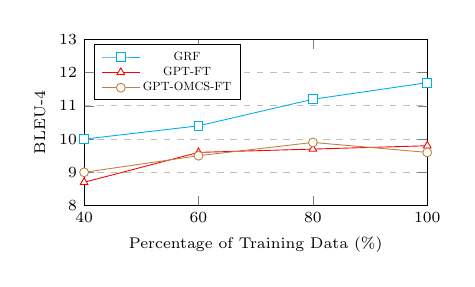
\begin{tikzpicture}[scale=0.8]
\small
\begin{axis}[
    title={},
    width=200pt,
    height=120pt,
    xlabel={Percentage of Training Data ($\%$)},
    ylabel={BLEU-4},
    xmin=40, xmax=100,
    ymin=8, ymax=13,
    xtick={40,60,80,100},
    ytick={8,9,10,11,12,13},
    yticklabel style={font=\scriptsize},
    xticklabel style={font=\scriptsize},
    xlabel style = {font=\scriptsize},
    ylabel style = {font=\scriptsize},
    legend pos=north west,
    legend style={nodes={scale=0.6, transform shape}},
    ymajorgrids=true,
    grid style=dashed
]

\addplot[
    color=cyan,
    mark=square*,
    mark options={fill=white},
    ]
    coordinates {
    (40,10.0)(60,10.4)(80,11.2)(100, 11.7)
    };
    \addlegendentry{GRF}

\addplot[
    color=red,
    mark=triangle*,
    mark options={fill=white},
    ]
    coordinates {
    (40,8.7)(60,9.6)(80,9.7)(100, 9.8)
    };
    \addlegendentry{GPT-FT}

\addplot[
    color=brown,
    mark=*,
    mark options={fill=white},
    ]
    coordinates {
    (40, 9.0) (60,9.5)(80,9.9)(100, 9.6)
    };
    \addlegendentry{GPT-OMCS-FT}

\end{axis}

\end{tikzpicture}
\caption{Performance with different amount of training data on the test set of $\alpha$NLG.}
\label{fig:amount}
\end{figure}



\begin{figure}[t]
\centering
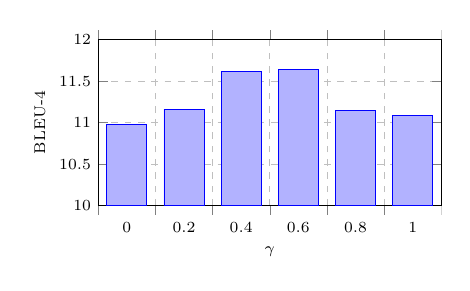
\begin{tikzpicture}[scale=0.8]
\small
\begin{axis}[
    title={},
    width=200pt,
    height=120pt,
    xlabel={$\gamma$},
    ylabel={BLEU-4},
    yticklabel style={font=\scriptsize},
    xticklabel style={font=\scriptsize},
    xlabel style = {font=\scriptsize},
    ylabel style = {font=\scriptsize},
    ymin=10, ymax=12,
    xmin=-0.2, xmax=1,
    %enlargelimits=0.05,
    %xtick={0.0,0.2,0.4,0.6,0.8,1.0},
    ytick={10,10.5,11,11.5,12},
    legend pos=north west,
    ymajorgrids=true,
    grid style=dashed,
    ybar interval=0.7,
]

\addplot
    coordinates {
     (1,11.08) (0.8, 11.15) (0.6, 11.64) (0.4,11.62) (0.2,11.16) (0,10.98) (-0.2,0)
    };
    %\addlegendentry{GSF}

\end{axis}
\end{tikzpicture}
\caption{Effect of $\gamma$ in DMRF. Performance with different value of discount factor $\gamma$ on the test set of $\alpha$NLG.}
\label{fig:gamma}
\end{figure}

\begin{figure}[t]
    \centering
    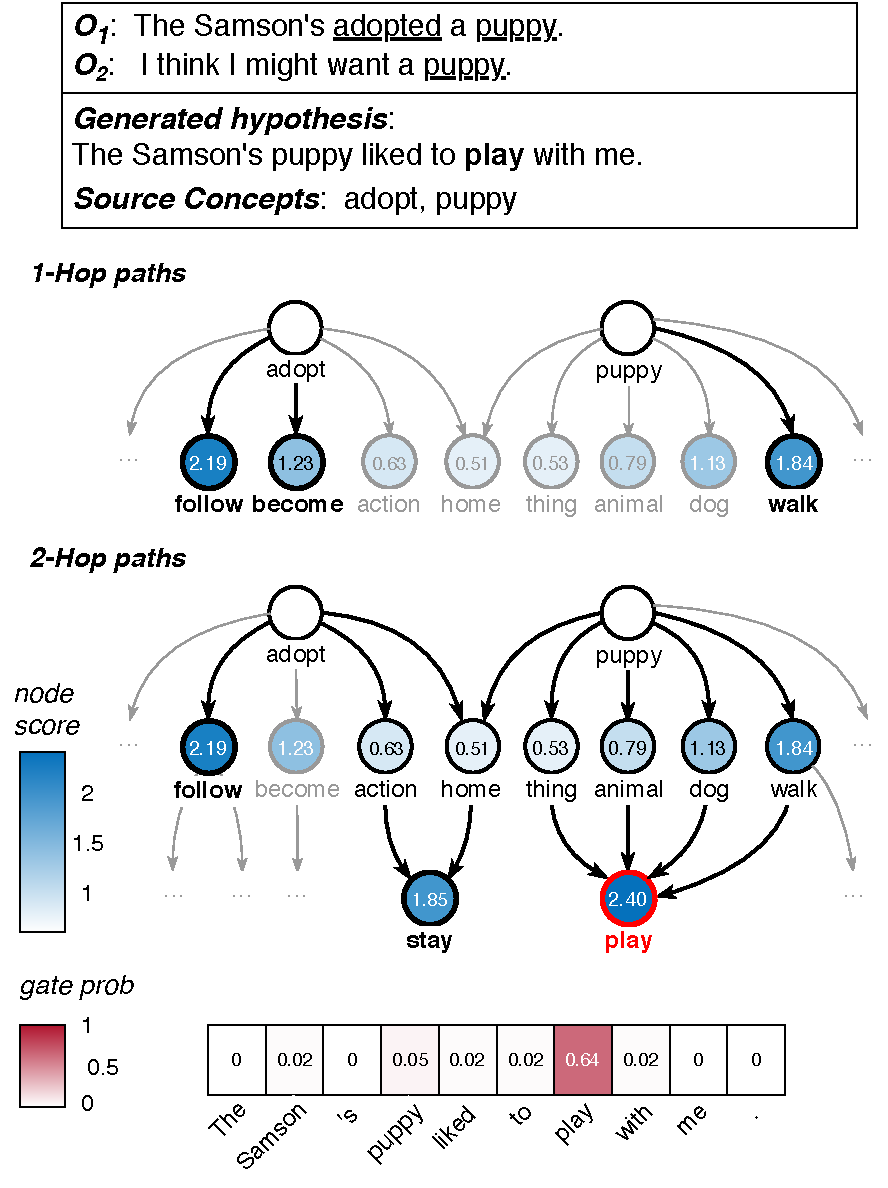
\includegraphics[width=0.9\columnwidth]{case_vis5.pdf}
    \caption{Visualization of a test case with inferred reasoning paths by our model. We highlight top-$3$ concepts with reasoning paths at \textbf{1-Hop} and \textbf{2-Hop} reasoning step respectively.}
    \label{fig:vis}
\end{figure}


\begin{table}[!t]
    \scriptsize
    \centering
    \setlength{\tabcolsep}{0.7mm}{
    \begin{tabular}{l l}
        \toprule[1.5pt]
        \multicolumn{2}{c}{\textbf{Story Ending Generation}} \\
        \midrule[1pt]
        \multirow{3}{*}[-4pt]{\textbf{Story Context}} & \textit{I wanted a simple bike for commuting.} \\
        {} & \textit{So I bought a \textcolor{myblue}{\textbf{cheap}} one on sale.} \\
        {} & \textit{But it didn't fit me properly.} \\
        {} & \textit{And it was uncomfortable to ride.} \\
        \midrule[1pt]
        \textbf{IE+GA} & So I decided to buy a new one. \\
        \textbf{GPT2-FT} & So I decided to buy a new bike. \\
        \textbf{GPT2-OMCS-FT} & So I decided to buy a bike from a bike shop instead. \\
        \textbf{GRF} & So I decided to get a more \textcolor{myorange}{\textbf{expensive}} bike. \\
        \midrule[1pt]
        \multirow{3}{*}[-4pt]{\textbf{Story Context}} & \textit{Ava made shakes for her kids on a \textcolor{myblue}{\textbf{hot}} summer day.} \\
        {} & \textit{She called them in from play, but they dallied.} \\
        {} & \textit{By time they came in, the shakes were almost \textcolor{myblue}{\textbf{melted.}}} \\
        {} & \textit{Ava blended in more \textcolor{myblue}{\textbf{ice}} cubes and refreshed them.} \\
        \midrule[1pt]
        \textbf{IE+GA} & Then she went home and ate them. \\
        \textbf{GPT2-FT} & Ava was proud of her kids for being so good at \\
        {} & cooking. \\
        \textbf{GPT2-OMCS-FT} & She was proud of her kids for being so thoughtful! \\
        \textbf{GRF} & Her kids thanked her profusely for helping them \\
        {} & \textcolor{myorange}{\textbf{cool}} off. \\
        \midrule[1pt]
        \multicolumn{2}{c}{\textbf{Abductive NLG}} \\
        \midrule[1pt]
        \textbf{Observation 1} & \textit{The Smith family went on a \textcolor{myblue}{\textbf{cruise}} for their summer} \\
        {} & \textit{vacation.} \\
        \textbf{Observation 2} & \textit{From then on, the Smiths went to the \textcolor{myblue}{\textbf{beach}} each}\\
        {} & \textit{summer instead.} \\
        \midrule[1pt]
        \textbf{GPT2-FT} & The Smith family had a great time on the beach. \\
        \textbf{GPT2-OMCS-FT} & The Smith family went to the beach. \\
        \textbf{COMeT-Emb-GPT2} & They didn't have a nice vacation. \\
        \textbf{GRF} & The Smith family got \textcolor{myorange}{\textbf{seasick}} on the cruise. \\
        \midrule[1pt]
        \textbf{Observation 1} & \textit{Nancy bought her dog a squeaky stuffed animal.} \\
        \textbf{Observation 2} & \textit{The dog had \textcolor{myblue}{\textbf{ripped}} the toy to shreds.} \\
        \midrule[1pt]
        \textbf{GPT2-FT} & Nancy found a toy that looked like a toy. \\
        \textbf{GPT2-OMCS-FT} & Nancy found a toy that looked like a toy. \\
        \textbf{COMeT-Emb-GPT2} & The squeaky stuffed animal was the first to come in. \\
        \textbf{GRF} & Nancy's dog \textcolor{myorange}{\textbf{scratched}} the stuffed animal. \\
        \midrule[1pt]
        \multicolumn{2}{c}{\textbf{Explanation Generation}} \\
        \midrule[1pt]
        \textbf{Statement} & \textit{\textcolor{myblue}{\textbf{Coke}} is made of \textcolor{myblue}{\textbf{alcohol}}.} \\
        \midrule[1pt]
        \textbf{GPT2-FT} & {Coke is a drink.} \\
        \textbf{GPT2-OMCS-FT} & {Coke is not a liquid.} \\
        \textbf{GRF} & {Coke is made from \textcolor{myorange}{\textbf{corn}}.} \\
        \midrule[1pt]
        \textbf{Statement} & \textit{She \textcolor{myblue}{\textbf{cut}} up a \textcolor{myblue}{\textbf{blanket}}.} \\
        \midrule[1pt]
        \textbf{GPT2-FT} & A blanket is not sharp enough to cut. \\
        \textbf{GPT2-OMCS-FT} & A blanket is too small to be cut. \\
        \textbf{GRF} & Blankets are too \textcolor{myorange}{\textbf{soft}} to be cut. \\
        
        \bottomrule[1.5pt]
    \end{tabular}}
    \caption{Case study on the test set of three datasets. Words in  \textcolor{myblue}{blue} denote source concepts in the input contexts while words in \textcolor{myorange}{orange} are the associated concepts generated by the GRF. }
    \label{tab:case_study}
\end{table}

\subsection{Impact of the Size of Training Data}

To demonstrate the complementary performance gain of utilizing relational paths besides textual modeling, we sample different fractions of training data of $\alpha$NLG for training and evaluate on the original test set. We compare our method with knowledge-agnostic finetuning of the GPT-2 model and the commonsense-enhanced GPT-2 post-trained on OMCS. As shown in Figure \ref{fig:amount}, our model achieves consistent performance gains against the chosen baselines with different amount of training data, which demonstrates the generalization ability of the proposed model with the aid of structural relation knowledge.



\subsection{Effectiveness of Dynamic Multi-Hop Reasoning}

We demonstrate the effectiveness of the multi-hop reasoning module through both quantitative and qualitative analysis. 

We investigate the impact of the hyper-parameter $\gamma$ that controls the information flow in the multi-hop reasoning module. 
% by the performance on the test set of abductive NLG. 
As shown in Figure \ref{fig:gamma}, the maximum performance is obtained when $\gamma$ is around $0.4$ and $0.6$. When $\gamma\rightarrow 0$, the multi-hop reasoning module reduces to local scoring of each concept and ignores evidence accumulated on the paths. While $\gamma\rightarrow 1$,
the node score increases monotonically along the paths %without any decay to the information flow 
which also hinders the model's ability to select the correct concept. Therefore, we set $\gamma=0.5$ for all the main results of our model.

To qualitatively assess the ability of the dynamic reasoning module, we visualize a test case on $\alpha$NLG with top-ranked concepts and scored reasoning paths. As shown in Figure \ref{fig:vis}, at the first hop the reasoning module starts from the source concepts ``\textit{adopt}'' and ``\textit{puppy}'' and assigns higher scores to neighbouring concepts which are verbs considering the generated context. At the second hop the module utilizes more plausible evidences along 2-hop reasoning paths and selects ``\textit{play}'' ($g_t=0.64$) which is more reasonable given both the observations.

%We also qualitatively assess the reasoning module by a test case on $\alpha$NLG with visualized reasoning paths inferred by our model. As shown in Figure \ref{fig:vis}, our model generates a reasonable hypothesis that follows the context of $O_1$ while explains the motives of $O_2$. Specifically, our reasoning module generates ``play'' with the highest node score by gathering related evidence through two-hop reasoning when direct connections to this salient concept do not exist on the graph. 
%It verifies that our model can effectively perform multi-hop reasoning to reach the salient target concept when direct connections to the concept do not exist.

%\begin{comment}
%As shown in Figure \ref{fig:vis}, blue nodes denote the zero-hop source concepts in the input and orange nodes denote the generated concept with gate probability over $0.5$. In Figure \ref{fig:case1}, the model generates ``\textcolor{myorange}{market}'' mainly by gathering related concepts in the input and aggregate evidence though the one-hop flow. In Figure \ref{fig:case2}, the generated ``\textcolor{myorange}{play}'' is mainly contributed by the two-hop flow starting from attributes of ``\textcolor{myblue}{puppy}'' such as ``\textcolor{mygreen}{dog}'' and `` \textcolor{mygreen}{animal}'' when direct connection is not available.
%\end{comment}


%We provide more generated examples from different models in the Appendix.
\subsection{Case Study}

We provide some test cases on three datasets in Table \ref{tab:case_study} and observe that: \textbf{I.} Baseline models tend to generate general cases while the GRF is able to generate more specific concepts by exploring the plausible relations between concepts. For example in the first case, the GRF generates ``expensive'' which is the antonym of ``cheap'' under the story context. \textbf{II.} Baseline models sometimes fail to identify the transition of the narrative as shown in the third case where the GRF generates ``seasick'' as a plausible explanation for the transition from ``cruise'' to ``beach''. \textbf{III.} The GRF generates proper attributes of the source concepts in the input context with the aid of external commonsense knowledge as shown in the last two cases of explanation generation.






\section{Conclusion}

We present Generation with Multi-Hop Reasoning Flow that reasons over structured commonsense knowledge during text generation. %Compared to previous transfer-based approaches to integrate commonsense knowledge into the pre-trained models, 
The proposed method leverages both the structural and semantic information of the external knowledge base by performing dynamic multi-hop reasoning on the relational paths. We conduct extensive experiments and empirically show that our method outperforms existing approaches that integrate commonsense knowledge to pre-trained language models on three text generation tasks. We also demonstrate the interpretability of our method with inferred reasoning paths that provide rationale to the generated results.
 
\section*{Acknowledgments}

This work was jointly supported by the NSFC projects (key project with No. 61936010 and regular project with No. 61876096), and the Guoqiang Institute of Tsinghua University with Grant No. 2019GQG1. We thank THUNUS NExT Joint-Lab for the support.

\bibliography{emnlp2020}
\bibliographystyle{acl_natbib}



\end{document}
